\documentclass[journal]{IEEEtran}

\usepackage[pdftex]{graphicx}
\usepackage[cmex10]{amsmath}
\usepackage{algorithmicx}
\usepackage{array}

\usepackage{amssymb,mathrsfs}
\usepackage{times}
\usepackage{color}
\usepackage{subfig}
\usepackage{cite}
\usepackage{multirow,tabularx}
\usepackage[ruled,lined]{algorithm2e}
\usepackage[compatible]{algpseudocode} 

\usepackage{wasysym}
\usepackage{stackrel}
\usepackage{tikz}
\usetikzlibrary{matrix,arrows,decorations.pathreplacing,automata,positioning,decorations.pathmorphing}
\usepackage{float}
\usetikzlibrary{shapes.multipart}
\newcommand{\myunit}{1 cm}
\tikzset{
    node style sp/.style={draw,circle,minimum size=\myunit},
    node style ge/.style={circle,minimum size=\myunit},
    arrow style mul/.style={draw,sloped,midway,fill=white},
    arrow style plus/.style={midway,sloped,fill=white},
}
\renewcommand{\algorithmiccomment}[1]{\textit{// #1}}
\renewcommand{\algorithmicrequire}{\textbf{Input:}}
\renewcommand{\algorithmicensure}{\textbf{Output:}}
\DeclareMathOperator*{\argmin}{arg\,min}

\newtheorem{theorem}{{\bf Theorem}}
\newtheorem{lemma}{{\bf Lemma}}
\newtheorem{proposition}{Proposition}
\newtheorem{corollary}{{\bf Corollary}}
\newtheorem{claim}{{\bf Claim}}
\newtheorem{problem}{{\bf Problem}}
\newtheorem{example}{{\bf Example}}
\newtheorem{definition}{{\bf Definition}}
\newtheorem{remark}{{\bf Remark}}



\newtheorem{fact}{Fact}
\newtheorem{obs}{Observation}



\newcommand{\net}{\mathcal{N}}
\newcommand{\netnodes}{V}
\newcommand{\netedges}{E}

\newcommand{\compgraph}{\mathcal{G}}
\newcommand{\compnodes}{\Omega}
\newcommand{\compedges}{\Gamma}
\newcommand{\prenodes}[1]{\Phi_{\uparrow}(#1)}
\newcommand{\sucnodes}[1]{\Phi_{\downarrow}(#1)}
\newcommand{\head}[1]{head(#1)}
\newcommand{\tail}[1]{tail(#1)}
\newcommand{\distance}{\mathtt{d}} \newcommand{\edgewt}{\mathtt{W}} \newcommand{\processingwt}{\mathtt{P}} 

\newcommand{\setofpaths}{\Sigma}
\newcommand{\pathstart}[1]{\mathsf{start}(#1)}
\newcommand{\pathend}[1]{\mathsf{end}(#1)}


\newcommand{\red}[1]{\textcolor{red}{#1}}
\newcommand{\new}[1]{#1}

\newcommand{\mincost}{\textsf{MinCost}}
\newcommand{\mindelay}{\textsf{MinDelay}}
\newcommand{\delaydecision}{\textsf{DelayDecision}}
\newcommand{\costdecision}{\textsf{CostDecision}}
\newcommand{\embedding}{\mathcal{E}}
\newcommand{\setofembeddings}{\mathbb{E}}
\begin{document}

\title{Optimal Embedding of Functions for In-Network Computation:
  Complexity Analysis and Algorithms}

\author{Pooja Vyavahare,~\IEEEmembership{} Nutan
  Limaye,~\IEEEmembership{} and~D.~Manjunath,~\IEEEmembership{Senior
    Member,~IEEE}
  \thanks{Pooja Vyavahare and D.~Manjunath are with the Deptt. of
    Elecl. Engg., and Nutan Limaye is with the Deptt.~ of Comp.
    Sc.~\& Engg. of IIT Bombay.}  \thanks{Email addresses are
    \{vpooja,dmanju\}@ee.iitb.ac.in and {nutan}@cse.iitb.ac.in }
  \thanks{This work was supported in part by DST projects SR/SS/EECE/0139/2011, ITRA/15(64)/Mobile/USEAADWN/01, and was
    carried out in the Bharti Centre for Communication at IIT Bombay.}
}

\maketitle

\begin{abstract}
  We consider optimal distributed computation of a given function of
  distributed data. The input (data) nodes and the sink node that
  receives the function form a connected network that is described by
  an undirected weighted network graph. The algorithm to compute the
  given function is described by a weighted directed acyclic graph and
  is called the computation graph. An embedding defines the
  computation communication sequence that obtains the function at the
  sink. Two kinds of optimal embeddings are sought, the embedding
  that---(1)~minimizes delay in obtaining function at sink, and
  (2)~minimizes cost of one instance of computation of function. This
  abstraction is motivated by three applications---in-network
  computation over sensor networks, operator placement in distributed
  databases, and module placement in distributed computing.

  We first show that obtaining minimum-delay and minimum-cost
  embeddings are both NP-complete problems and that cost minimization
  is actually MAX SNP-hard. Next, we consider specific forms of the
  computation graph for which polynomial time solutions are
  possible. When the computation graph is a tree, a polynomial time
  algorithm to obtain the minimum delay embedding is described. Next,
  for the case when the function is described by a layered graph we
  describe an algorithm that obtains the minimum cost embedding in
  polynomial time. This algorithm can also be used to obtain an
  approximation for delay minimization. We then consider bounded
  treewidth computation graphs and give an algorithm to obtain the
  minimum cost embedding in polynomial time.
\end{abstract}

\begin{keywords}
  In-network function computation; operator placement; graph
  embedding;
\end{keywords}
\IEEEpeerreviewmaketitle

\section{Introduction}
\label{sec:intro} 

\subsection{Background}

Efficient computing of functions of distributed data is of interest in
many applications, most recently in sensor networks \cite{Giridhar05}
and in programming models for distributed processing of large data
sets, e.g., MapReduce \cite{Dean04} and Dryad \cite{Isard07}.

Consider a typical sensor network scenario where sensor nodes measure
and store environment variables and form a distributed database. These
nodes also have computing and communication capabilities and can form
a connected network. A sink node, also called terminal or receiver, is
interested in one or more functions of this distributed data rather
than in the raw data itself. Conventional examples for such functions
are maximum, minimum, mean, parity, and histogram
\cite{Giridhar05}. More sophisticated functions are also easily
motivated, e.g., spatial and temporal correlations, spectral
characteristics of the data (that may be obtained by performing FFT on
the data), and filtering operations on the raw data in sensor
networks. A naive approach to obtain the required function(s) of the
distributed data at the sink would be to collect the raw data at the
sink and have it perform the computation. Alternatively, since the
nodes have computation capability, it could possibly be more efficient
to push the computation into the network, i.e., use a distributed
computation scheme over the communication network.  Our interest is in
the latter approach---efficient `in-network computation' of the
required function.

Several measures of efficiency of computation may be defined. Total
energy expended in obtaining one sample of the function is a possible
measure. Delay from the time at which the data is available at the
sources to the time at which the function value is available at the
sink is a second possible measure. If the data at each of the sources
were to be a stream, then the rate at which the function values are
available at the sink is a third possible measure. In this paper we
consider only the first two measures above---cost of computation and
delay in computation. Thus our focus is on algorithms that find an
computation and communication (routing) sequence to compute a target
function on a given network that minimize the delay or the cost.  The
target functions are assumed to belong to the class of functions that
are computed using a scheme that can be represented as directed
acyclic graphs (DAGs). The following example illustrates our intent.

Consider a network of  nodes,  of which collect measurement data
from their environment. Let  be data sample available at node
 () at time  and let  be the function of
interest.  can be computed using the schema of
Fig.~\ref{fig:r-of-t}a. Each edge in this directed graph represents an
intermediate value in the computation of  and each node
corresponds to an operation that is to be performed on its inputs. The
communication network over which  is to be computed is shown in
Fig.~\ref{fig:r-of-t}b as a weighted undirected graph. In the example
all the edges have unit weight. Two possible computation and
communication schemes are shown in
Figs.~\ref{fig:r-of-t}c,d. We see that the scheme in
Fig.~\ref{fig:r-of-t}c has a lower cost than that in
Fig.~\ref{fig:r-of-t}d.

Several flavors of in-network function computation exist in the
literature. A randomly deployed multihop wireless network of noise
free links is considered in
\cite{Giridhar05,Giridhar06,Khude05,Kamath14}. They determine
asymptotic achievable rates at which different symmetric functions
like minimum, maximum and type vector may be computed. An identical
objective is addressed in
\cite{Gallager88,Kushilevitz98,Feige00,Newman04,Goyal05} for single
hop networks with noisy links and in \cite{Ying07,Dutta08} for
multihop wireless networks with noisy links. When the nodes are in a
 grid and communicate over wireline or
wireless links, \cite{Karamchandani11} obtains the time and number of
transmissions required to compute a function. Randomized gossip
algorithms \cite{Boyd05,Shah09}, where a random sequence of node-pairs
exchange data and perform a specific computation is used in
\cite{Mosk-Aoyama06,Ayaso08,Bodas11} for function computation. The
interest is in time for all nodes to converge to the specified
function. Another stream of work considers computing of specific
functions using network coding and designs the communication networks
to maximize the computation rate
\cite{Ramamoorthy10,Appuswamy11,Rai12}. None of the above consider
minimum cost function computation. Further, to the best of our
knowledge, only \cite{Shah13} considers computation of arbitrary
functions in finite size networks; the interest there is on maximizing
the rate of computation.

\begin{figure}[tbp]
  \centering
\subfloat[]{
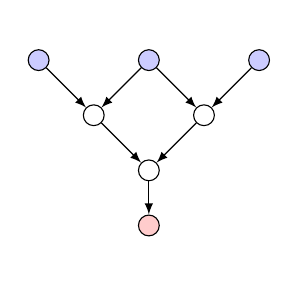
\begin{tikzpicture}[>=latex,scale=0.7]
 \scriptsize
 \tikzstyle{every node} = [circle,draw=black]
 \node (a) at (-2,0) [fill=blue!20] {};
 \node (b) at (0,0) [fill=blue!20] {};
 \node (c) at (2,0) [fill=blue!20] {};
 \node (d) at (-1,-1)[font=\tiny]  {};
 \node (e) at (1,-1) [font=\tiny]{};
 \node (f) at (0,-2)[font=\tiny] {};
 \node (g) at (0,-3) [fill=red!20]{};
 \node at (-2,0.4) [draw=none]{};
 \node at (0,0.4) [draw=none]{};
 \node at (2,0.4) [draw=none]{};
 \node at (0,-3.4) [draw=none]{};
\draw [->] (a) -- (d) ;
 \draw [->] (b) -- (d) ;
 \draw [->] (b) -- (e) ;
 \draw [->] (c) -- (e) ;
 \draw [->] (d) -- (f) ;
 \draw [->] (e) -- (f) ;
 \draw [->] (f) -- (g) ;
 
 \end{tikzpicture}
}
\hspace*{10pt}
\subfloat[]{
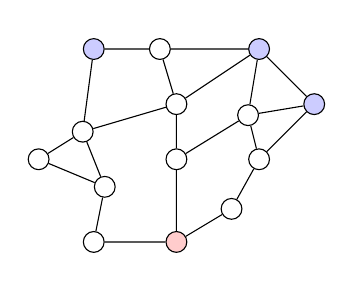
\begin{tikzpicture}[>=latex,scale=0.7]
  \scriptsize
  \tikzstyle{every node} = [circle,draw=black]
  \node (a) at (-2,0) [fill=blue!20]  {};
  \node (b) at (-0.8,0) {};
  \node (c) at (1,0)  [fill=blue!20]  {};
  \node (d) at (-2.2,-1.5) {};
  \node (e) at (-0.5,-1) {};
  \node (f) at (0.8,-1.2) {};
  \node (g) at (1,-2)  {};
  \node (h) at (0.5,-2.9) {};
  \node (i) at (-0.5,-2) {};
  \node (j) at (-1.8,-2.5) {};
  \node (k) at (-0.5,-3.5) [fill=red!20] {};
  \node (l) at (-2,-3.5){};
  \node (m) at (2,-1)[fill=blue!20] {};
  \node (n) at (-3,-2){};
\draw [-] (a) -- (b) -- (c) -- (m) --(f) --(c) -- (e)  --(i) -- (k);
  \draw [-] (a) -- (d) -- (n) -- (j) -- (l) --(k);
  \draw [-] (m) -- (g) -- (h) --(k);
  \draw [-] (e) -- (d) -- (j);
  \draw [-] (i) -- (f) -- (g);
  \draw [-] (b) -- (e);
\node at (a) [draw=none,above] {};
  \node at (c) [draw=none,above] {};
  \node at (m) [draw=none,above] {};
  \node at (-0.5,-3.9) [draw=none] {};
\end{tikzpicture}
} 


\subfloat[]{
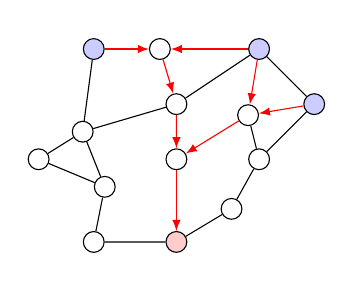
\begin{tikzpicture}[>=latex,scale=0.7]
  \scriptsize
  \tikzstyle{every node} = [circle,draw=black]
  \node (a) at (-2,0) [fill=blue!20]  {};
  \node (b) at (-0.8,0) {};
  \node (c) at (1,0)  [fill=blue!20]  {};
  \node (d) at (-2.2,-1.5) {};
  \node (e) at (-0.5,-1) {};
  \node (f) at (0.8,-1.2) {};
  \node (g) at (1,-2)  {};
  \node (h) at (0.5,-2.9) {};
  \node (i) at (-0.5,-2) {};
  \node (j) at (-1.8,-2.5) {};
  \node (k) at (-0.5,-3.5) [fill=red!20] {};
  \node (l) at (-2,-3.5){};
  \node (m) at (2,-1) [fill=blue!20] {};
  \node (n) at (-3,-2) {};
\draw [-] (c) -- (e)  ;
  \draw [-] (a) -- (d) -- (n) -- (j) -- (l) --(k);
  \draw [-] (m) -- (g) -- (h) --(k);
  \draw [-] (e) -- (d) -- (j);
  \draw [-] (f) -- (g);
  \draw [-] (c) -- (m) ;
\draw [->,color=red] (a) -- (b)  ;
  \draw [->,color=red] (b) -- (e) ;
  \draw [->,color=red] (e) -- (i) ;
  \draw [->,color=red] (i) -- (k) ;
  \draw [->,color=red] (m) -- (f) ;
  \draw [->,color=red] (c) -- (b) ;
  \draw [->,color=red] (c) -- (f) ;
  \draw [->,color=red] (f) -- (i) ;
\node at (a) [draw=none,above] {};
  \node at (c) [draw=none,above] {};
  \node at (m) [draw=none,above] {};
  \node at (-0.5,-3.9) [draw=none] {};
\end{tikzpicture}
} 
\hspace*{10pt}
\subfloat[]{
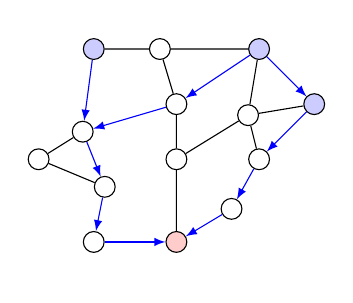
\begin{tikzpicture}[>=latex,scale=0.7]
  \scriptsize
  \tikzstyle{every node} = [circle,draw=black]
  \node (a) at (-2,0) [fill=blue!20]  {};
  \node (b) at (-0.8,0) {};
  \node (c) at (1,0)  [fill=blue!20]  {};
  \node (d) at (-2.2,-1.5) {};
  \node (e) at (-0.5,-1) {};
  \node (f) at (0.8,-1.2) {};
  \node (g) at (1,-2)  {};
  \node (h) at (0.5,-2.9) {};
  \node (i) at (-0.5,-2) {};
  \node (j) at (-1.8,-2.5) {};
  \node (k) at (-0.5,-3.5) [fill=red!20] {};
  \node (l) at (-2,-3.5){};
  \node (m) at (2,-1) [fill=blue!20] {};
  \node (n) at (-3,-2) {};
\draw [-] (a) -- (b) -- (c) --(f) -- (m);
  \draw [-]  (d) -- (n) ;
  \draw [-] (i) -- (f) -- (g);
  \draw [-] (b) -- (e);
  \draw [-] (e)  --(i) -- (k);
  \draw [-] (n) -- (j);
\draw [->,color=blue] (a) -- (d)  ;
  \draw [->,color=blue] (d) -- (j);
  \draw [->,color=blue] (j) -- (l) ;
  \draw [->,color=blue] (l) -- (k) ;
  \draw [->,color=blue] (c) -- (e)  ;
  \draw [->,color=blue] (e) -- (d) ;
  \draw [->,color=blue] (c) -- (m) ;
  \draw [->,color=blue] (m) -- (g) ;
  \draw [->,color=blue] (g) -- (h) ;
  \draw [->,color=blue] (h) -- (k) ;
\node at (a) [draw=none,above] {};
  \node at (c) [draw=none,above] {};
  \node at (m) [draw=none,above] {};
  \node at (-0.5,-3.9) [draw=none] {};
\end{tikzpicture}
} 
  \caption{Computation of function .
    (a) A schema to compute  (b) Communication Network (c) Implementation 1 (d) Implementation 2}
  \label{fig:r-of-t}
\end{figure}

Rather than arithmetic operations to perform a function computation,
the nodes in Fig.~\ref{fig:r-of-t}a could correspond to operations
required to execute a database query and the directed edges would
represent the flow of the results of the operations. In this case the
graph of Fig.~\ref{fig:r-of-t}a is called a query graph. The input
data to this query graph could be from a distributed database, which
in turn could be a sensor network; in this case the graph in
Fig.~\ref{fig:r-of-t}b would represent the interconnection among the
units of the distributed database and some other nodes that may be
available for computation. In this context performing an efficient
query requires that the `operator placement' be efficient. Efficient
operator placement is addressed in
\cite{Bonfils04,Srivastsava05,Abrams05,Pietzuch06,Ying08,Wen13} all of
which assume that the query graph is a tree. While
\cite{Wen13,Pietzuch06,Bonfils04} develop heuristics based algorithms
for efficient operator placement when the query graph is a tree,
algorithms with formal analyses are available in
\cite{Srivastsava05,Abrams05,Ying08}. Although \cite{Phatak10}
considers a non-tree query graph, only heuristic algorithms are
provided.

Going back in the literature, we see that the `module placement'
problem for distributed processing from the 1980s has a flavor similar
to in-network computation and operator placement problems; see e.g.,
\cite{Stone77,Bokhari81,MaryLo88,Bokhari88,Fernandez-Baca89}. In this
case the nodes of Fig.~\ref{fig:r-of-t}a correspond to the modules of
a program and a directed edge  implies that module  calls
module  during execution.  Further, the graph of
Fig.~\ref{fig:r-of-t}a is called a \textit{call graph.} The nodes of
Fig.~\ref{fig:r-of-t}b represent the processors on which the modules
of the program need to be executed and the edges represent the inter
processor links. The cost structure for this problem is more
complex. The execution cost is specified for each module-processor
pair and there is also an inter processor communication cost over an
edge that in turn depends on the modules placed at the ends of the
edge. The objective is to place the modules on the processors such
that the total cost of execution is minimized.  The first centralized
algorithm for optimal module placement when the call graph is a
directed tree was given in \cite{Bokhari81} and that for -trees was
given in \cite{Fernandez-Baca89}. \cite{Stone77} showed that the
problem can be efficiently solved for a two processor system by using
network flow algorithms and \cite{MaryLo88} uses a similar approach to
develop heuristic algorithms for a general call graph.

From the preceding discussion we see that the objectives of, and hence
the solution techniques for, efficient in-network computation,
operator placement and module placement all have a very similar
theme---embedding (a formal definition is provided in
Section~\ref{sec:prelims}) a graph representing a computation schema
on a connected weighted graph representing a network of
processors. Much of the literature on such problems assumes that the
graph describing the function is a tree. This is clearly very
restrictive because the computation schema for a very large class of
useful computable functions cannot be described by a tree and are more
generally described by a DAG, e.g., fast Fourier transform (FFT),
sorting, any polynomial function of input data, and any function of
Boolean data.  MapReduce, the popular cloud computing paradigm, also
has a DAG representation and is discussed in some detail in
Example~\ref{ex:mapreduce} in Section~\ref{sec:layered-graph}.

\subsection{Organization of the Paper}

Our interest is in computing arbitrary functions that have a specific
algorithmic representation and the communication network is an
arbitrary network and not a random wireless network. (We reiterate
that although we assume the in-network computation scenario to anchor
the discussion, our results are also directly applicable to the
operator and module placement scenarios.)  Further, we do not seek to
specifically maximize the computation throughput; rather, our interest
is in minimizing the cost or delay in a `one shot' computation of the
function. As we mentioned before, two measures of efficiency are used
in this paper---cost of computation and delay in computation. Our
results on minimum cost embedding can be used to maximize computation
throughput when used in the algorithms developed in \cite{Shah13}.

Given an arbitrary function via its DAG description and an arbitrary
network over which this function is to be computed, our first interest
is to analyze the complexity of finding the optimal computation and
communication scheme that will compute the function in the
network. While much of the literature claims that this problem is
NP-complete (for the case of minimizing cost), to the best of our
knowledge a formal proof is not available; the literature eventually
leads to a citation to a private communication in \cite{Bokhari81}. In
Section~\ref{sec:hardness} we prove that in general, both the minimum
cost and the minimum delay embedding problems are NP-complete.

Some structure in the DAG can be exploited to provide polynomial time
algorithms for our problems. If the DAG is a tree, which is the
assumption in much of the extant literature, the minimum cost
embedding is similar to shortest path algorithms
\cite{Ying08,Shah13}. To the best of our knowledge, minimum delay
embeddings are not considered in the literature and in
Section~\ref{sec:tree} we provide a polynomial time algorithm to find
the minimum delay embedding when the computation schema is a tree.

Next we consider two large classes of computation graphs---(1)~layered
graphs, (2)~bounded treewidth graphs. We derive the motivation for
layered graphs from distributed data processing frameworks like
MapReduce \cite{Dean04} and Dryad \cite{Isard07}.  In
Section~\ref{sec:layered-graph} we provide a polynomial time algorithm
to find the minimum cost embedding when the DAG is a layered
graph. This same algorithm also obtains an approximation for the
minimum delay embedding.

In Section~\ref{sec:treewidth}, we show that the algorithm from
Section~\ref{sec:layered-graph} can find the minimum cost embedding
when the DAG is a bounded treewidth graph.  
The notation and the
formal problem definition is described in the next section.

In Section~\ref{sec:change_computation}, we describe an update
mechanism when there is perturbation in the DAG and we conclude with a
discussion in Section~\ref{sec:discuss}.

\section{Preliminaries}
\label{sec:prelims}

The communication network is represented by an undirected connected
graph  with  being the set of
 nodes and  being the set of  edges. The elements of
 are denoted by  Each edge
 has a non negative weight 
associated with it. The weight could, for example, correspond to
transmission time of a bit on the link, or the energy required to
transmit one bit on the link or something more abstract.  For a given
 and any  let  be the
weight of the minimum cost path from  to  Let  be the  distance matrix.  Of the
 nodes in , there are  source nodes denoted by  Source node  generates data
 denote  A sink node 
requires to obtain a function  of the data.

We assume that schema to compute  is given
and is represented by a directed acyclic graph  where  is the set of  nodes
and  is the set of  edges. The nodes in 
are denoted by  and correspond to
operations that need to be performed on the input data to the node and
the outgoing edges denote the flow of the result of these
operations. Thus each edge in  represents a sub-function
of the inputs. The sources in the computation graph are denoted by
nodes  with node 
corresponding to source  node  is the sink that
receives the function 

The direction on the edges in  represent the direction of
the flow of the data.  Each edge 
has a non negative weight  associated with
it which could correspond to the number of bits used to represent the
intermediate function. 

Since  is a directed acyclic graph there is a partial
order associated with its vertices. If  then the function at  cannot be computed until
the function at  is computed and the result forwarded to
 Let  and  denote,
respectively, the immediate predecessors and successors of vertex
 i.e.,  and 
A processing cost (delay) function  is used to capture the cost (delay) of
performing a particular operation on a particular vertex of the
network. Now we define the embedding of  on  as
follows.
\begin{definition}
  \label{def:embedding}
  An embedding of a computation graph  on a communication
  network  is a many-to-one function  which satisfies the following conditions. 
  \begin{enumerate}
  \item  for 
  \item 
  \end{enumerate}
\end{definition}
In this definition of embedding each node in the computation graph is
mapped to a single node in the network graph and the edge
 is mapped to the shortest path
between  and  Alternate
definitions of an embedding are possible, e.g., an edge in
 can be mapped to more than one path in  while
satisfying some continuity constraints; this is the definition of an
embedding in \cite{Shah13}. 

An embedding defines a computation and communication
sequence in  to obtain  at the sink. Let 
be the set of all embeddings of  in  which
follow Definition~\ref{def:embedding}.  The weight functions  and
 can be treated as, respectively, the communication and the
processing delays in  for computing and communicating the
sub-functions leading to computation of  We can define the delay in
computing a sub-function by a node  in the
embedding  as
 
Recall that  is the length of the shortest path between
vertices  thus the first term here corresponds to
the delay in obtaining all the operands at node 
and the second term corresponds to the processing delay at the
node. Setting the delay at the sources to zero, i.e.,
 for all  we can
recursively calculate the delay of each vertices of  on
 The delay  of an embedding  is defined
 as the delay of the sink, i.e., 

This leads us to the first problem that we consider in this
paper:~Find an embedding  such that the delay of
the embedding is minimum among all the embeddings for a given
 and  i.e., solve the
optimization problem



Alternatively, considering the weight functions   and
 as cost of communication and computation, e.g., the
energy cost, the cost of an embedding can be defined as

We can then find an embedding  such that the cost
of the embedding is minimum among all the embeddings for a given
 and  i.e., solve the
optimization problem


The following example illustrates the preceding problems and the
system set up. 

\begin{example}
 \label{ex:delaycostcomp}
  Consider a computation graph 
  and communication network  shown in
  Fig.~\ref{fig:sysmodel}.  The labels of each vertex in both the
  graphs are shown in Fig.~\ref{fig:sysmodel}.  The processing
  cost (delay) for sources is assumed to be zero and for other
  vertices of  it is assumed to be unity.
\begin{figure}[tbp]
\centering
\subfloat[]{
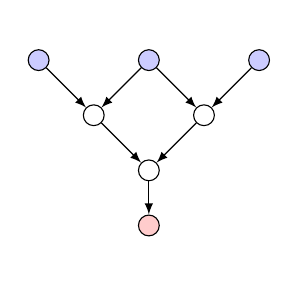
\begin{tikzpicture}[>=latex,scale=0.7]
 \scriptsize
 \tikzstyle{every node} = [circle,draw=black]
 \node (a) at (-2,0) [fill=blue!20] {};
 \node (b) at (0,0) [fill=blue!20] {};
 \node (c) at (2,0) [fill=blue!20] {};
 \node (d) at (-1,-1)[font=\tiny]  {};
 \node (e) at (1,-1) [font=\tiny]{};
 \node (f) at (0,-2)[font=\tiny] {};
 \node (g) at (0,-3) [fill=red!20]{};
 \node at (-2,0.4) [draw=none]{};
 \node at (0,0.4) [draw=none]{};
 \node at (2,0.4) [draw=none]{};
 \node at (0,-3.4) [draw=none]{};
 \node at (d) [draw=none,right=4pt] {};
 \node at (e) [draw=none,right=4pt] {};
 \node at (f) [draw=none,right=4pt] {};
\draw [->] (a) -- (d) ;
 \draw [->] (b) -- (d) ;
 \draw [->] (b) -- (e) ;
 \draw [->] (c) -- (e) ;
 \draw [->] (d) -- (f) ;
 \draw [->] (e) -- (f) ;
 \draw [->] (f) -- (g) ;
\end{tikzpicture}
}
\subfloat[]{
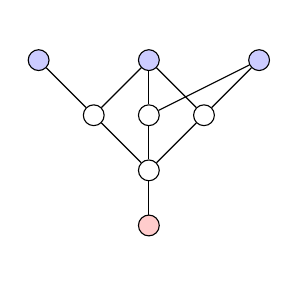
\begin{tikzpicture}[>=latex,scale=0.7]
  \scriptsize
  \tikzstyle{every node} = [circle,draw=black]
\node (a) at (-2,0) [fill=blue!20] {};
 \node (b) at (0,0) [fill=blue!20] {};
 \node (c) at (2,0) [fill=blue!20] {};
 \node (d) at (-1,-1)  {};
 \node (e) at (1,-1) {};
 \node (f) at (0,-1) {};
 \node (g) at (0,-2) {};
 \node (h) at (0,-3) [fill=red!20]{};
 \node at (-2,0.4) [draw=none]{};
 \node at (0,0.4) [draw=none]{};
 \node at (2,0.4) [draw=none]{};
 \node at (0,-3.4) [draw=none]{};
 \node at (d) [draw=none,right] {};
 \node at (f) [draw=none,right] {};
 \node at (e) [draw=none,right] {};
 \node at (g) [draw=none,right] {};
\draw [-] (a) -- (d)node [draw=none, midway,left] {};
 \draw [-] (d) -- (g)node [draw=none, midway,left] {} ;
 \draw [-] (b) -- (d) node [draw=none, midway,left] {};
 \draw [-] (c) -- (f)node [draw=none, pos=0.05,left] {};
 \draw [-] (b) -- (e)node [draw=none, pos=0.2,right] {}; 
 \draw [-] (e) -- (g)node [draw=none, midway,right] {};
 \draw [-] (c) -- (e) node [draw=none, midway,right] {};
 \node at (-0.2,-0.5) [draw=none] {};
 \draw [-] (b) -- (f);
\node at (-0.2,-1.5) [draw=none] {};
 \draw [-] (f) -- (g);
\node at (-0.2,-2.5) [draw=none] {};
 \draw [-] (g) -- (h);
\end{tikzpicture}
} 
\vspace*{6pt}
\subfloat[]{
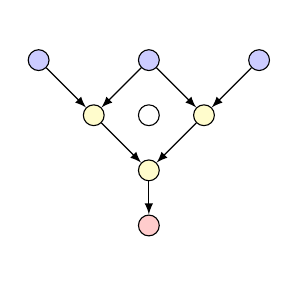
\begin{tikzpicture}[>=latex,scale=0.7]
  \scriptsize
  \tikzstyle{every node} = [circle,draw=black]
\node (a) at (-2,0) [fill=blue!20] {};
 \node (b) at (0,0) [fill=blue!20] {};
 \node (c) at (2,0) [fill=blue!20] {};
 \node (d) at (-1,-1) [fill=yellow!20] {};
 \node (e) at (1,-1) [fill=yellow!20] {};
 \node (f) at (0,-1) {};
 \node (g) at (0,-2) [fill=yellow!20] {};
 \node (h) at (0,-3) [fill=red!20]{};
 \node at (-2,0.4) [draw=none]{};
 \node at (0,0.4) [draw=none]{};
 \node at (2,0.4) [draw=none]{};
 \node at (0,-3.4) [draw=none]{};
 \node at (-0.5,-1) [draw=none] {};
\node at (0.4,-1) [draw=none] {};
\node at (1.5,-1) [draw=none] {};
 \node at (0.5,-2) [draw=none] {};
\draw [->] (a) -- (d);
 \draw [->] (b) -- (d);
 \draw [->] (b) -- (e);
 \draw [->] (c) -- (e);
 \draw [->] (d) -- (g);
 \draw [->] (e) -- (g);
 \draw [->] (g) -- (h);
\end{tikzpicture}
} 
\subfloat[]{
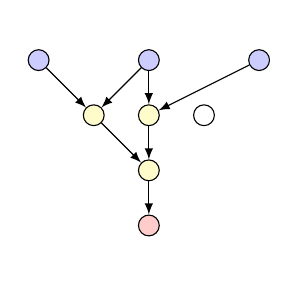
\begin{tikzpicture}[>=latex,scale=0.7]
  \scriptsize
  \tikzstyle{every node} = [circle,draw=black]
\node (a) at (-2,0) [fill=blue!20] {};
 \node (b) at (0,0) [fill=blue!20] {};
 \node (c) at (2,0) [fill=blue!20] {};
 \node (d) at (-1,-1) [fill=yellow!20] {};
 \node (e) at (1,-1) {};
 \node (f) at (0,-1) [fill=yellow!20] {};
 \node (g) at (0,-2)[fill=yellow!20] {};
 \node (h) at (0,-3) [fill=red!20]{};
 \node at (-2,0.4) [draw=none]{};
 \node at (0,0.4) [draw=none]{};
 \node at (2,0.4) [draw=none]{};
 \node at (0,-3.4) [draw=none]{};
 \node at (-0.5,-1) [draw=none] {};
\node at (0.4,-1.1) [draw=none] {};
 \node at (1.4,-1) [draw=none] {};
\node at (0.5,-2) [draw=none] {};
\draw [->] (a) -- (d);
 \draw [->] (b) -- (d);
 \draw [->] (d) -- (g);
 \draw [->] (g) -- (h);
 \draw [->] (b) -- (f);
 \draw [->] (f) -- (g);
 \draw [->] (c) -- (f);
\end{tikzpicture}
} 
    \caption{(a). Computation graph  for } (b). Communication Network  The
    numbers near the edges represent the weights on them.
    (c). Minimum delay embedding  
(d). Minimum cost embedding
    
    \label{fig:sysmodel}
  \end{figure}
  An embedding  of  on  will have
   and
   Now consider two embeddings
   such that  and
   These are shown in
  Figs.~\ref{fig:sysmodel}c~and~\ref{fig:sysmodel}d.

  Using \eqref{eq:embedding-cost}, it is easy to verify that
   and  The delays in the
  embedding  are:  and finally
   Similarly,
   Observe that the delay of  is
  lower among the two but its cost is higher than that of
   
\end{example}


Now we present an example which shows that the difference between the
delay obtained by the solution of \mincost\ problem and that of the
\mindelay\ problem can be of the order of the number of sources in the
network.
\begin{figure}[tbp]
\subfloat[]{
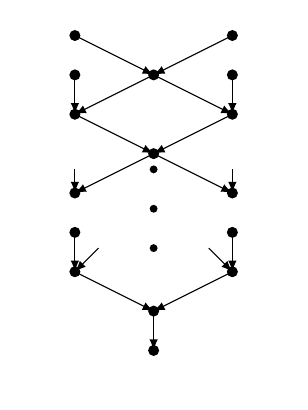
\begin{tikzpicture}[>=latex]
\footnotesize
 \foreach \x in {-1,1}{
  \foreach \y in {2,1.5,1,-0.5,0,-1}{
   \fill (\x,\y) circle (0.07cm);
   }
 }
\foreach \y in {1.5,0.5}{
  \fill (0,\y) circle (0.07cm);
  \draw [->] (0,\y) -- (-1,\y-0.5);
  \draw [->] (0,\y) -- (1,\y-0.5);
  }  
\foreach \x in {-1,1}{
  \draw [->] (\x,2) -- (0,1.5);
  \draw [->] (\x,1) -- (0,0.5);
  \draw [->] (\x,1.5) -- (\x,1);
  \draw [->] (\x,-0.5) -- (\x,-1);
  \draw [->] (\x,-1) -- (0,-1.5);
  }
\foreach \y in {0.3,-0.2,-0.7} {
 \fill (0,\y) circle (0.05cm);
 }
\fill (0,-1.5) circle (0.07cm);
\fill (0,-2) circle (0.07cm);
\draw [->] (0,-1.5) -- (0,-2);
\draw [->] (-0.7,-0.7) --(-1,-1);
 \draw [->] (0.7,-0.7) -- (1,-1);
 \draw [->] (-1,0.3) -- (-1,0);
 \draw[->] (1,0.3) -- (1,0);
 
 \node at (-1.3,2) [draw=none] {};
 \node at (1.3,2) [draw=none] {};
 \node at (-1.3,1.5) [draw=none] {};
 \node at (1.3,1.5) [draw=none] {}; 
 \node at (-1.5,-0.5) [draw=none] {};
 \node at (1.3,-0.5) [draw=none] {};
 \node at (0,-2.3) [draw=none] {};
\node at (-1.3,1) [draw=none] {};
 \node at (1.3,1) [draw=none] {};
 \node at (0,1.7) [draw=none] {};
 \node at (0,0.7) [draw=none] {};
 \node at (-1.5,-1) [draw=none] {};
 \node at (1.5,-1) [draw=none] {};
 \node at (0.5,-1.6) [draw=none] {};
 \end{tikzpicture}
}
\hspace*{10pt}
  \subfloat[]{
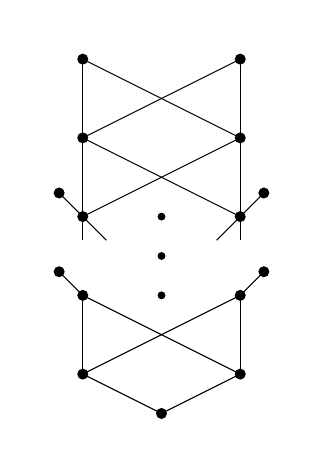
\begin{tikzpicture}[>=latex]
\footnotesize
 \foreach \x in {-1,1} {
  \foreach \y in {2,1,0} {
   \fill (\x,\y) circle (0.07cm);
  }
 }
 \foreach \x in {-1,1} {
  \foreach \y in {2,1,-1} {
    \draw [-] (\x,\y) -- (\x,\y-1); 
   }
 }
\draw [-] (-1,0) -- (-1,-0.3);
 \draw [-] (1,0) -- (1,-0.3);
 \draw [-] (-1,0) -- (-0.7,-0.3);
 \draw [-] (1,0) -- (0.7,-0.3);
 
  \foreach \y in {2,1,-1} {
   \draw [-] (-1,\y) -- (1,\y -1);
   \draw [-] (1,\y) -- (-1,\y-1);
   } 
  \foreach \y in {-1,0,-0.5} {
   \fill (0,\y) circle (0.05cm);
   } 
\fill (-1.3,0.3) circle (0.07cm);
   \fill (1.3,0.3) circle (0.07cm);
   \draw [-] (-1.3,0.3) -- (-1,0);
   \draw [-] (1.3,0.3) -- (1,0);
   \fill (-1.3,-0.7) circle (0.07cm);
   \fill (1.3,-0.7) circle (0.07cm);
   \draw [-] (-1.3,-0.7) -- (-1,-1);
   \draw [-] (1.3,-0.7) -- (1,-1);
\node at (-1,2.3) [draw=none] {};
   \node at (1,2.3) [draw=none] {};
   \node at (-1.6,0.3) [draw=none] {};
   \node at (1.6,0.3) [draw=none] {};
   \node at (-1.3,-0.4) [draw=none] {};
   \node at (1.3,-0.4) [draw=none] {};
   \node at (0,-2.8) [draw=none] {};
\foreach \x in {-1,1} {
    \foreach \y in {-1,-2} {
     \fill (\x,\y) circle (0.07cm);
     }
     }
     \draw [-] (-1,-2) -- (0,-2.5);
     \draw [-] (1,-2) -- (0,-2.5);
     \fill (0,-2.5) circle (0.07cm);
\node at (-1.1,1.5) [draw=none] {};
     \node at (1.3,1.5) [draw=none] {};
     \node at (-0.4,1.95) [draw=none] {};
     \node at (0.4,1.95) [draw=none] {};
\node at (-1.1,-1.5) [draw=none] {};
     \node at (1.3,-1.5) [draw=none] {};
     \node at (-0.4,-1.05) [draw=none] {};
     \node at (0.4,-1.05) [draw=none] {};
\node at (-0.7,0.3) [draw=none] {};
     \node at (0.7,0.3) [draw=none] {};
     \node at (-1.1,0.6) [draw=none] {};
     \node at (1.1,0.6) [draw=none] {};
     \node at (-0.7,-2.3) [draw=none] {};
     \node at (0.7,-2.3) [draw=none] {};
\node at (-1.3,1) [draw=none] {};
     \node at (1.3,1) [draw=none] {};
     \node at (-1.3,0) [draw=none] {};
     \node at (1.3,0) [draw=none] {};
     \node at (-1.4,-2) [draw=none] {};
     \node at (1.4,-2) [draw=none] {};
 \end{tikzpicture}
}
  \caption{Illustrating Example~\ref{ex:compare}. (a). Computation graph with 
    sources and a sink.  (b). Communication network.}
  \label{fig:delaycost_diff}
\end{figure}
\begin{example}
  \label{ex:compare}
  Consider the computation graph  and a network graph
   as shown in
  Figs.~\ref{fig:delaycost_diff}a and b respectively. The labels of
  the vertices are shown in the figure and the numbers near the edges
  of  represent the weight of that edge. Note that the structure
  between  to  and  to  is repeated in the network
  graph  times. Let us call this structure as  We assume that
  the weights on the edges of  are all one and the
  processing costs are zero for sources and for all other vertices it
  is assumed unity. Any embedding  of  on
   will have  and  Consider an embedding
   such that  Let us compute the
  cost of this embedding. Note that the total cost of the embedding is
   times the cost coming from the structure  plus the weight of
  edge  The cost due to embedding of  is the sum of the
  weights of edges  and the processing
  costs at  Hence the cost of the embedding is
   Similarly the
  delay of this embedding is  Now consider another embedding  such that
   The cost and delay for this embedding can be computed in a
  similar fashion to obtain  and 
  It can be shown that the first embedding  is the
  solution of \mincost\ where as  is the solution of
  \mindelay\ problem of  on  If we use the solution
  of \mincost\ to get the solution of \mindelay\ then the difference
  would be  which is of the
  order of the number of sources in the graph.
\end{example}



\section{Hardness of Embedding}
\label{sec:hardness}


We begin by considering \mindelay. First consider the case when there
is no processing delay, i.e.,
 in the network and the
computation graph is unweighted, i.e., 
 
The delay of the embedding in this case is the delay of the longest
embedded path from any source to the sink in  Let
 be the delay of the minimum delay path between
source  and the sink  in  Then the delay of any
embedding of  on  which follows the conditions of
Definition~\ref{def:embedding} has to be more than the delay on the
longest of all the minimum delay paths from sources to sink. In other
words, 
Now consider an embedding  which maps all the
intermediate vertices of  to the sink in  The delay
of this embedding will be 
Comparing it with  tells us that the embedding
 minimizes the delay. Hence \mindelay\ is easy to
solve if there are no processing delays and  is
unweighted.

Now we analyze the hardness of \mindelay\ and \mincost\ for arbitrary
 and  and show that the both the optimization
problems are NP-hard. We prove the hardness of the optimization
problems by proving that the corresponding decision versions are
NP-hard. The decision versions of the \mindelay\ and \mincost\ are
defined as follows:

\begin{definition}
  For a given  and a positive
  number  the decision version of the \mindelay\ problem outputs
  \textit{``yes"} if there exists an embedding  of
   on  such that  and outputs
  \textit{``no"} if no such embedding exists.
\end{definition}

\begin{definition} 
  For a given  and a positive
  number  the decision version of the \mincost\ problem outputs
  \textit{``yes"} if there exists an embedding  of
   on  such that  and outputs
  \textit{``no"} if no such embedding exists.
\end{definition}

Note that if one can solve the optimization version of \mindelay\
(resp. \mincost) problem in time, say  then using the solution of
that problem we can solve the corresponding decision version in time
 Hence the original optimization problem is atleast as hard as
its decision version. This implies that if we just prove that the
decision version of the \mindelay (resp. \mincost) is NP-hard then the
optimization version is also NP-hard. We now proceed to prove that the
decision version of our optimization problems are indeed NP-complete.

\begin{theorem}
\label{thm:delay}
The decision version of \mindelay\ problem is NP-complete.
\end{theorem}

\begin{proof}
  We first prove that the decision version of \mindelay\ is NP-hard by
  giving a reduction from the NP-complete problem \textit{Precedence
    Constraint Scheduling with fixed mapping (PCS-FM)}\cite{Garey79}.

  PCS-FM problem is defined as follows. Given a set of tasks  with
  a partial order  on it, task  having length  a set  and  processors, find a schedule  of tasks on the
  processors which meets an overall deadline  maps each
   to a particular processor  and obeys
  the precedence constraint that if  then
   To the best of our knowledge the
  hardness of PCS-FM problem has not been proved in the literature and
  we provide the proof of NP-completeness of PCS-FM in Appendix~\ref{sec:PCS-FM}. 

  We first give a reduction from an instance  of PCS-FM to an instance
  of \mindelay\  where
   and  are the computation and communication graphs
  respectively. The set  is to be mapped to
   under any embedding  and
   are the communication and processing delay of the
  network. Note that the set of tasks  along with the partial order
  creates a DAG  and we define  We
  define  to be a complete graph on  processors. Let  and  The transmission delay  between
  any two vertices of  is taken as 
  and  for all  Finally 

  We have to prove that there is a schedule  of  which
  finishes in time  if and only if there is an embedding
   of  with delay  The forward direction is easy to prove. If there is a
  schedule of  which finishes in  time and maps a
  task  to a processor  then we can create an embedding of
   which maps the same vertex  to a vertex  Note that because  and  the conditions of Definition~\ref{def:embedding} are met in
  this embedding. The delay of any vertex  in this
  embedding will be at most the time at which the task  finishes in
  the schedule  plus the number of times edges in  are
  used because of the same precedence order. Hence the delay of this
  embedding will be 

  To complete the proof we need to prove that if there is an embedding
   of  of delay  then there
  is a schedule  of  which finishes in time  We will create a schedule  from the
  embedding  If a vertex  is mapped to
  a vertex  then in the schedule  also the
  task  is executed by processor  Because  and
   the tasks in  are mapped to  in
  this schedule also. Let the total number of edge uses in this
  embedding be  Note that  in any embedding where 
  are the number of vertices in graph  The total
  transmission delay in the embedding is  Recall that
  the processing delays are all  hence the delay of the embedding
  can be written as  It
  is easy to verify that the time required by the schedule  to
  complete is  This proves that the decision
  of \mindelay\ is NP-hard.

  Given an instance of \mindelay\ problem an embedding 
  can be guessed non-deterministically and checked whether
   in polynomial time. Thus the decision version
  of \mindelay\ problem is in NP and our reduction proves that it is
  in fact NP-complete.
\end{proof}

We now look at the problem of approximating the \mindelay\ problem. We
say that a polynomial time approximation algorithm has a performance
guarantee  if it outputs a feasible solution of the problem
which has delay at most  times the optimal solution.  We prove
the following:

\begin{theorem}
  \label{thm:delayapprox}
  Unless P=NP, an instance of the \mindelay\ problem with
   and with unit processing
  delays and unit weights on the edges of  does not have
  a polynomial-time approximation algorithm with performance guarantee
  strictly less than  if its solution is greater than 
\end{theorem}


\begin{proof}
  Note that while proving the hardness of \mindelay\ we first reduced
  an instance of a PCS problem to an instance of a PCS-FM problem and
  then we reduced PCS-FM to \mindelay\ problem. Let 
  and  be the deadline achieved by the optimal and a
  feasible solution of PCS problem respectively. Similarly, let
   and  be the deadline achieved by
  the optimal and a feasible solution of the PCS-FM problem. Finally,
  let  and  be the optimal and
  feasible solutions for \mindelay. While proving the NP-completeness
  of PCS-FM (in Appendix~\ref{sec:PCS-FM}) we showed that  We also showed that if a schedule of PCS problem
  achieves a deadline  then there is a schedule of
  PCS-FM with  Let PCS-FM have a
  polynomial-time approximation algorithm with solution
   By Observation~5.1 of
  \cite{Hoogeveen98} we know that the PCS problem does not have
  polynomial-time approximation algorithm with performance guarantee
  less than  Hence, 
  Substituting the relation between  and
   in the above equation we get, 
   Thus, 
   and 
  We now observe that  and hence  we can write,  and finally 
  Hence, unless P=NP, PCS-FM cannot have a polynomial time
  approximation algorithm with performance guarantee less than 
  While proving the hardness for \mindelay\ we showed that for any
  instance of PCS-FM with  we can get an instance of
  \mindelay\ problem with solution  such that
   Let
  \mindelay\ have a polynomial time approximation algorithm with
  solution  We know that
   Substituting the
  relation between  and  in the above
  expression we get,  and 
     This implies that
    
  Observe that, if  then  (because of the reduction) implies that
   So we get  This completes the proof.
\end{proof}

We now consider the decision version of \mincost.

\begin{remark}
  \label{rm:directed}
  Recall that the cost of an embedding  is computed using
  \eqref{eq:embedding-cost} which does not consider the direction on
  the edges of  It only considers the weight  on
  any edge of  Thus the cost of an embedding does not
  depend on the directions of the edges and the solution of \mincost\
  problem is same irrespective of whether the computation graph
   has directions or not.
\end{remark}

\begin{theorem}
  \label{thm:mincost}
  The decision version of the \mincost\ is NP-complete.
\end{theorem}

\begin{proof}
  We actually prove that the decision version of \mincost\ is NP-hard
  even when the processing costs are zero and the costs on the edges
  of  and  are all one. In this case the cost of the
  embedding  is given by 
  where  is the shortest distance between the vertices
  

  We prove the hardness of the decision version of \mincost\ by giving
  a reduction from the unweighted version of \textit{Multiterminal
    Cut} problem which is NP-complete \cite{Dahlhaus94}.
  Multiterminal Cut problem is defined as follows: Given an arbitrary
  graph  and
  a set  of 
  specified vertices, find the minimum number of edges  such that the removal of 
  from  disconnects each vertex in  from all
  the other vertices in 

  The cost of an embedding can be computed in polynomial time using
  \eqref{eq:embedding-cost}. Hence, given an instance of the decision
  version of the \mincost\ problem, one can guess an embedding in a
  non-deterministic way and check whether its cost is less than  or
  not in polynomial time. Thus the decision version of the \mincost\
  problem is in NP. To prove the NP-hardness of the problem we will
  first show a transformation of an instance of Multiterminal Cut
  problem  to an instance of the decision
  version of \mincost\  Then
  we will show that there exists a set of edges in  of
  size  which separates all the vertices of  from all other
  vertices in  if and only if there is an embedding 
  such that a vertex  is mapped to a vertex
   and has cost equal to 

  From  define an instance of decision version of \mincost\
   as follows: Let  be a complete graph on  where  and 
  Note that in this case  is undirected. Define
   and  such that a vertex 
  is mapped to  In other words,  distinct
  vertices of  are mapped to distinct vertices of
   Now we prove that there is an embedding  of
  cost  if and only if  has a Multiterminal Cut of size equal
  to 

  The ``if'' part is easy to see. If there is a minimum Multiterminal
  Cut  of size  which divides the vertex set
   into  disjoint subsets then define
   such that each vertex in  is
  mapped to  Then the cost of the embedding is the
  total number of edges which go from  to
   for  This is nothing but the size
  of the set  which is equal to 

  To complete the proof we need to show that if there is no minimum
  Multiterminal Cut of  of size  then there is no embedding
  (which maps the vertices of  to vertices of  of
   with cost  Let us assume that there is no minimum
  Multiterminal Cut of  of size  but there is an embedding
  for  with cost  It implies that there is a mapping of
   on  different vertices of  such that
   is mapped to  Let us denote all the vertices of
   that are mapped to  by  The cost of
  the embedding is equal to the number of edges between sets
   and  for  which is equal to
   Now it is easy to see that if we divide the vertices of
   in  disjoint subsets such that all the vertices
  in  are in the same set then we can create a
  Multiterminal Cut of the graph  which has cost
  exactly  But this contradicts our assumption. Hence if there is
  an embedding function  for  of cost  then there
  is a Multiterminal Cut of  of same size. This proves that the
  decision version of \mincost\ is NP-hard when the computation graph
  is undirected. From Remark~\ref{rm:directed}, thus the decision
  version of \mincost\ with directed computation graph is also
  NP-hard.

  So far, we have not considered any weight functions. From
  \cite{Dahlhaus94} we know that the Multiterminal Cut problem for
  weighted graphs is also NP-complete. And a simple modification in
  our reduction will prove that decision version of \mincost\ problem
  with weight functions is also NP-hard.
\end{proof}

It is also shown in \cite{Dahlhaus94} that Multiterminal Cut problem
is MAX SNP-hard. To prove any problem being MAX SNP-hard it is
sufficient to give a linear reduction to it from a known MAX SNP-hard
problem. The linear reduction is defined as follows:

\begin{definition}
  Let  and  be two optimization problems. Then we
  say that  linearly reduces to  if there are two
  polynomial time algorithms  and two constants  such that
\begin{enumerate}
  \item Given an instance  of  with an optimal cost
     an algorithm  produces an instance
     of  such that the cost of an
    optimal solution for 
    is at most  i.e., 
  \item Given  and any solution  of
     there is an algorithm  which produces a solution
     of  such that 
  \end{enumerate}
\end{definition}

Note that in the proof of Theorem~\ref{thm:mincost} we use polynomial
time algorithms to reduce an instance  of the Multiterminal Cut
problem to an instance  of the \mincost\ problem and we proved
that  We can also get a
solution of  from a solution of  and vice versa with
parameters  Hence the reduction we used to prove
that \mincost\ is NP-complete is in fact a linear reduction of
Multiterminal Cut problem to \mincost. We thus have the following
corollary.

\begin{corollary}
  Problem \mincost\ is MAX SNP-hard and hence does not have any
  polynomial time approximation scheme unless P=NP \cite{Arora92}.
\end{corollary}



The NP-hardness of \mincost\ can also be proved by reduction from
another well known NP-complete problem -clique \cite{Garey79}.  The
-clique problem is defined as follows: Given an arbitrary graph
 and a positive integer  check whether
 has a clique
(or a complete subgraph) of size  Since we know that the
-clique problem is complete \cite{Downey99}, the reduction
from it also implies that \mincost\ does not have any fixed-parameter
tractable algorithm and is also hard for 

A variation of \mincost\ is considered in \cite{Fernandez-Baca89} in
that the communication costs (computed as  in this
paper) are not necessarily zero if  Further, the source and the sink nodes are not
fixed like in this paper. The key complexity result is Lemma~2.1 which
shows that their variation of \mincost\ with zero-one communication
costs is NP-complete by reducing it from the planar -SAT
problem. Their proof technique does not allow the communication to be
necessarily zero if  For
non zero-one communication costs, \cite{Fernandez-Baca89} also gives a
polynomial time algorithms for their variation when  is a
partial -tree and \textit{almost trees with parameter } 

As is the case with many NP-complete problems our problems also become
tractable when  has special structures. We consider three
such structures that have wide applications---the tree, layered graphs
and bounded treewidth graphs. These are considered next.

\section{ is a Tree}
\label{sec:tree}
Many functions that are useful on sensor networks, e.g., average,
maximum, minimum etc., can be represented by directed tree
graphs. Operations that are required to resolve many database queries
can also be represented as directed tree structures.  The trees
representing a  is from a class of trees that have a set
of leaf vertices whose in-degree is zero and a root vertex whose
out-degree is zero. We consider a tree structured  such
that all the leaf vertices represent the sources of data and the root
acts as the sink which wants to know the final function value. Recall
that we label all the vertices in  as
 Also  and
   represent the predecessor and successor
  vertices of the vertex  It is easy to
verify that in this type of tree structured computation graph, every
vertex (except the root) has only one successor vertex, i.e., for any
 (except the root) the set 
is a singleton set. The set  is null, where
 is the root and there is a unique path from each source to
the sink.

As we have mentioned earlier, \cite{Ying08} and \cite{Shah13} adapt,
respectively, the Bellman-Ford and the Dijkstra shortest path
algorithms to solve \mincost\ when  is a tree. In the
following we will describe Algorithm~\ref{algo:tree} that solves
\mindelay\ when  is a tree.

\textbf{Algorithm overview:} Algorithm~\ref{algo:tree} is a
centralized algorithm which assumes knowledge of the all-pair shortest
path delay matrix  of the communication network 
The optimal embedding is computed by iterating through all the edges
of the computation graph  For an edge
 of  the algorithm computes the
optimal delay of the path leading to the vertex  from
sources via  for all possible mappings of the vertex
 in the network. The delay till any vertex  is the
maximum of the optimal delays of all the paths reaching to 
plus the processing delay at that vertex. Once the optimal delay for
the sink node is computed, the algorithm backtracks to find the
optimal mapping of all the other vertices.


\textbf{Algorithm Description:} In each iteration the
Algorithm~\ref{algo:tree} maintains the following data structures: 
\begin{algorithm}
  \caption{Optimal embedding algorithm to solve \mindelay\ for tree
    graphs}
  \label{algo:tree}
 
  \begin{algorithmic} [1]
    \REQUIRE{Network graph ,   Weight function , Tree computation graph    Weight function  Cost function } 
  
    \ENSURE{Embedding  with minimum delay under  and } 
    \STATE  \COMMENT{ distance matrix for }
    \BlankLine
    \COMMENT{Initialization of tables}
    \STATE   \;
    \STATE   \; \FOR{ \KwTo }  \FORALL{}
    \STATE  \;
    \STATE  \;
    \STATE  \;
    \ENDFOR
    \ENDFOR
\FOR{ \KwTo } \FORALL{}
    \FORALL{}
    \STATE  \;
    \ENDFOR
    \STATE  \;
    \STATE  \;
    \ENDFOR
    \ENDFOR
    \STATE  \;\STATE  \;
    \COMMENT{Backtracking}
    \FOR{ \KwTo }
    \STATE  \;
    \ENDFOR
  \end{algorithmic}
\end{algorithm}



\begin{enumerate}
\item  It is the delay associated with edge
   and vertex  when
   and  are mapped to vertex  and
   respectively.
\item  It is the optimal delay of the path leading to vertex
   (via  when it is mapped to  The algorithm also stores the mapping of vertex 
  in  corresponding to this value.
\end{enumerate}

After initializing these data structures to zero (lines ) the
algorithm completes in the following two steps.

\textbf{Lines --} This is the iteration over all the sources in
   As the mapping of source  is
  fixed to source  here we just calculate the minimum
  delay required to reach to all the vertices from the source 
  Note that the processing delay at the source is zero, i.e.,
  
  
\textbf{Lines --} This is the main loop of the algorithm which
  runs over all the remaining vertices of  starting from
   to  In each iteration  is
  updated for all possible mappings of vertices
   (lines --. The function
   is computed by adding the following delay terms.
\begin{itemize}
  \item  This is the processing delay
    associated with the vertex  when it is performed at
    vertex 
  \item 
    This is the communication delay associated with the edge
     when mapped to  and 
    respectively.
 \end{itemize}
Then  is updated in line  Note that
  is the minimum delay
 till the vertex  when it is mapped to  This is
 equivalent to the first term in right hand side of
 ~\eqref{eq:nodedelay} (Section~\ref{sec:prelims}, Page 3). This along
 with the processing delay  gives the
 delay of the vertex  when mapped to  As mentioned
 earlier the algorithm also stores the mapping  in  which
 minimizes the 
 
\textbf{Lines --} Once all the delays are computed the algorithm
  computes the delay at the sink vertex  (as the mapping of
   is fixed to  in embedding  and finds the
  mapping of vertices of  on  which gives this value
  by backtracking from the sink to the sources.


\subsubsection{Analysis of Algorithm~\ref{algo:tree}}

\begin{theorem}
  \label{thm:mindelay_tree}
  Algorithm~\ref{algo:tree} solves \mindelay\ when  is a
  tree and runs in  time. Recall that  and  are the
  number of vertices in  and  respectively.
\end{theorem}

\begin{proof}
  We give the proof of correctness of Algorithm~\ref{algo:tree} only
  when the computation graph is unweighed. The proof can easily be
  extended to the case when there are weights on the edges of
   Recall that the delay of an embedding is defined
  recursively over all the vertices of  starting from the
  sink vertex. It is sufficient to prove that at any iteration  the
  algorithm computes the optimal delay of embedding the path from any
  source  to an intermediate vertex 
  via  for all possible embeddings of 
  And then at the end it chooses the fixed mapping of the sink
   and traces back the optimal paths from sink to all the
  sources via the intermediate vertices. We will prove this
  inductively.

  Let  be the assignment of  in  and at
  any iteration  for some  The optimal path from any source  for  to its successor vertex  is
  just the shortest path distance between  and the vertex to
  which  will eventually be mapped. This is equal
  to  It is easy to verify that in the
  algorithm (line  this value is stored in  data structure for all  Assuming that
  the optimal delays till the  run are calculated by the
  algorithm and stored in s we will show that at  run the
  algorithm computes the optimal delay. The optimal delay of the path
  from sources to  via  is given by
   
  where,  is the optimal delay of the path till
   The optimal delay  can further be
  expanded and written in terms of the delay of its predecessors as:
  
 Substituting value of  in  we get

Recall the line  of Algorithm~\ref{algo:tree} which computes
   This is
  nothing but the last two terms of the right hand side of
  \eqref{eq:gfinal} when  and  Now
  observe the line  of Algorithm~\ref{algo:tree} which computes
   where  is the
  optimal delay of the path leading to  via its predecessor
   The optimal delay of the path  for  Hence
  Algorithm~\ref{algo:tree} indeed computes the optimal delay of the
  path leading to  via  for all
  possible mappings  of  and
  stores it in  at iteration 

  Recall that  is a tree thus the total number of edges in
  it are  and Algorithm~\ref{algo:tree} is executed once for each
  edge. In each iteration it computes the delay of an edge for all
  possible mappings of its end points which requires  (line 
  time where  is the number of vertices in  Then it adds the
  delay to the delay of its predecessors and chooses the one with
  minimum value ( in line  which requires 
  time. Hence the time to complete one iteration is  The total time complexity of Algorithm~\ref{algo:tree} is
  
\end{proof}

\section{ is a Layered Graph}
\label{sec:layered-graph}

We now consider the case when  is a layered graph.  An
example of a layered computation graph is shown in
Fig.~\ref{fig:layered}. We assume that there are  layers and number
of vertices in each layer is at most  The vertices at layer 
are labelled  The
directed graph has edge  only if  Here we also assume that all the sources are at
layer one and there is only one sink  on the last layer.
\begin{figure}[tbp]
  \centering
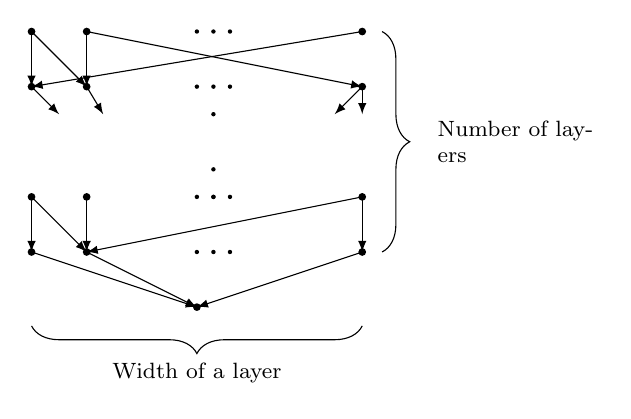
\begin{tikzpicture}[>=latex,scale=0.7]
\footnotesize
\foreach \x in {-3,-2,3} {
  \foreach \y in {-1,0,2,3} {
    \fill (\x,\y) circle (0.07cm);
  }  
}    
\foreach \x in {0,0.3,0.6} {
  \foreach \y in {-1,0,2,3} {
    \fill (\x,\y) circle (0.04cm);
  }  
} 
\foreach \y in {0,0.5,1.5}
  \fill (0.3,\y) circle (0.04cm);
\fill (0,-2) circle (0.07cm);

\draw[->] (-3,3) -- (-3,2);
\draw[->] (-3,3) -- (-2,2);  
\draw[->] (-2,3) -- (-2,2);     
\draw[->] (3,3) -- (-3,2);
\draw[->] (-2,3) -- (3,2);
\draw[->] (-3,2) -- (-2.5,1.5);
\draw[->] (-2,2) -- (-1.7,1.5);
\draw[->] (3,2) -- (2.5,1.5);
\draw[->] (3,2) -- (3,1.5);
\draw[->] (-3,0) -- (-3,-1);
\draw[->] (-3,0) -- (-2,-1);  
\draw[->] (-2,0) -- (-2,-1);     
\draw[->] (3,0) -- (-2,-1);
\draw[->] (3,0) -- (3,-1);
\draw[->] (-3,-1) -- (0,-2);
\draw[->] (-2,-1) -- (0,-2);
\draw[->] (3,-1) -- (0,-2);
\node at (0,-2.4){};    
\draw [decorate,decoration={brace,amplitude=10pt},xshift=-4pt,yshift=0pt]
(3.5,3) -- (3.5,-1) node [black,midway,xshift=0.6cm,text width=2cm,right] {Number of layers };
\draw [decorate,decoration={brace,amplitude=10pt},xshift=0pt,yshift=-4pt]
(3,-2.2) -- (-3,-2.2) node [black,midway,yshift=-0.6cm] {Width of a layer };
\end{tikzpicture}
  \caption{Layered computation graph}
  \label{fig:layered}
\end{figure}  


We derive our motivation for these kind of computation graphs from the
MapReduce application framework. In MapReduce framework each user
comes to a network of processors with a set of Map and Reduce
tasks. There is a precedence order between Map and Reduce tasks. Each
Reduce task cannot be started unless the processing of corresponding
set of Map tasks is finished. Each task takes predefined time to
finish and the outputs of the Map tasks are used by the corresponding
Reduce tasks. This dependency can be represented by a directed graph
with edges showing the dependency between the two tasks. The aim in
this setting is to embed the Map and Reduce tasks on the processors
such that the total time of computation and communication is
minimized. We explain our motivation with the following example from
\cite{Dean04}.

\begin{example}
  \label{ex:mapreduce}
  Consider a typical database query by a server (call it sink) to
  check the number of occurrences of different words in two large
  files which are available at two separate servers. The
  task of calculating the number of occurrences of each word inside
  the files can be divided into the following sub-tasks.
\begin{itemize}
  \item \textit{Splitting:} First the files are split into smaller
    sub-files such that each sub-file can be processed by a processor
    in the network.
  \item \textit{Mapping:} Each sub-file is then parsed to get the
    number of times each word occurred in it.
  \item \textit{Shuffling and reducing:} Once the count from each
    sub-file is available then the counts of one word are transported
    to one processor to compute the final count of that word. Each
    processor adds all the individual counts and results the final
    count of each word.
   \item \textit{Final result:} Finally the result is transported to
    the node which asked this query.
  \end{itemize}
Fig.~\ref{fig:mapreduce} represents a typical MapReduce data flow
  diagram for this problem. The aim is to determine the processors for
  each of the sub-tasks such that the time to answer the query at the
  sink is minimized. The whole process can be represented by a
  directed layered graph with each layer representing one sub-task and
  a vertex at a layer representing a particular sub-task. Observe that
  the edges in this graph are only between the consecutive layers and
  the operations at a vertex cannot start until the data from all its
  predecessors is available.
\begin{figure}[tbp]
    \centering
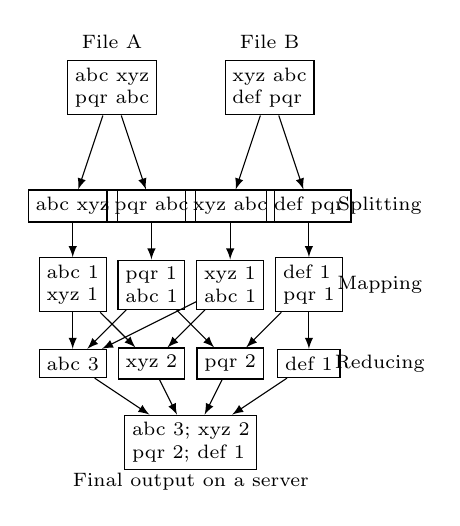
\begin{tikzpicture}[>=latex]
  \scriptsize
  \tikzstyle{ibox}=[draw=black,very thick,shape=rectangle,rounded corners=0.5em,inner sep=4pt,minimum height=2em,text badly centered];
\node[draw,align=left](a) at (-1,2) {abc xyz \\ pqr abc};
  \node[draw,align=left](b) at (1,2) {xyz abc \\ def pqr};
  \node at (-1,2.4) [draw=none,above] {File A};
  \node at (1,2.4) [draw=none,above] {File B};  
\node[draw,align=left](a1) at (-1.5,0.5) {abc xyz};
  \node[draw,align=left](a2) at (-0.5,0.5) {pqr abc};
  \node[draw,align=left](b1) at (0.5,0.5) {xyz abc};
  \node[draw,align=left](b2) at (1.5,0.5) {def pqr};
  \node at (2.4,0.5) [draw=none] {Splitting};
\draw[->] (a) -- (a1);
  \draw[->] (a) --(a2);
  \draw[->] (b) -- (b1);  
  \draw[->] (b) -- (b2);
\node[draw,align=left](a11) at (-1.5,-0.5) {abc 1 \\ xyz 1};
  \node[draw,align=left](a21) at (-0.5,-0.5) {pqr 1\\ abc 1};
  \node[draw,align=left](b11) at (0.5,-0.5) {xyz 1\\ abc 1};
  \node[draw,align=left](b21) at (1.5,-0.5) {def 1\\ pqr 1};
\node at (2.4,-0.5) [draw=none] {Mapping};
  \draw[->] (a1) -- (a11);
  \draw[->] (a2) --(a21);
  \draw[->] (b1) -- (b11);  
  \draw[->] (b2) -- (b21);
\node[draw,align=left](a12) at (-1.5,-1.5) {abc 3};
  \node[draw,align=left](a22) at (-0.5,-1.5) {xyz 2};
  \node[draw,align=left](b12) at (0.5,-1.5) {pqr 2};
  \node[draw,align=left](b22) at (1.5,-1.5) {def 1};
\node at (2.4,-1.5) [draw=none] {Reducing};
  \draw[->] (a11) -- (a12);
  \draw[->] (a11)--(a22);
  \draw[->] (a21) -- (a12);
  \draw[->] (a21) -- (b12);
  \draw[->] (b11) -- (a12);
  \draw[->] (b11) -- (a22);
  \draw[->] (b21) -- (b12);
  \draw[->] (b21) -- (b22);
  \node[draw,align=left] (t) at (0,-2.5) {abc 3; xyz 2\\ pqr 2; def 1};
  \node at (0,-3) [draw=none,align=center] {Final output on a server};
   \draw[->] (a12) -- (t);
  \draw[->] (a22) --(t);
  \draw[->] (b12) -- (t); 
  \draw[->] (b22) -- (t);
\end{tikzpicture}
   \caption{Sub-tasks and data flow diagram of a typical database query
      in MapReduce framework}
    \label{fig:mapreduce}
  \end{figure}  
\end{example}

\begin{algorithm}\caption{Optimal embedding algorithm for layered graphs}
\label{algo:layer}
 
  \begin{algorithmic} [1]
    \REQUIRE{Network graph ,   Weight function , Layered computation graph    Weight function  Cost function }  
  
    \ENSURE{Embedding  with minimum cost} \STATE  \COMMENT{ distance matrix for }
    \STATE  and   \COMMENT{ }
\STATE  and   \COMMENT{ }
\STATE  \COMMENT{ is the assignment of node  in optimal embedding}
    \BlankLine
    \COMMENT{Initialization of tables}
\STATE   \;
    \STATE   \; 

  \BlankLine
\FOR{ \KwTo }
    \FOR{ \KwTo }
      \FOR{ \KwTo }
    
      \STATE  \;\ENDFOR
      \STATE  \;\STATE  \; \ENDFOR
\ENDFOR
   \FOR{ \KwTo } \STATE  \;
                                      
  \ENDFOR
 \STATE  \;\STATE  \; \COMMENT{Backtracking}
  \FOR{ \KwTo }
     \STATE  \;
  \ENDFOR
\end{algorithmic}
\end{algorithm}


Now we present an algorithm which solves the \mincost\ problem for
layered graphs in polynomial time.

\textbf{Algorithm overview:} Like Algorithm~\ref{algo:tree},
Algorithm~\ref{algo:layer} also has two phases---a forward path and a
backward tracking. The forward path is a dynamic program that iterates
over all the layers of the computation graph. In the first iteration
it computes the optimal mappings of all the vertices of layer 
corresponding to a possible mapping of the vertices of layer  If a
vertex is a source vertex then its mapping is always fixed to the
corresponding source vertex in  Similarly, in iteration  it
computes the optimal mapping of vertices of layer  each
corresponding to a possible mapping of vertices of layer  It
also computes the optimal cost till layer  for every possible
mapping of vertices of layer  Once it reaches the last layer the
algorithm chooses the mapping of the vertices of last layer which
minimizes the overall cost and backtracks to get the corresponding
mappings of all the previous layers. 

\textbf{Algorithm Description:} Algorithm~\ref{algo:layer} iterates
over the layers in  and in each iteration it maintains the
following two data structures:
\begin{enumerate}
\item  the cost of embedding all the vertices till
  layer  when the vertices at layer  are placed at  and
  vertices of layer  are placed at  where  of size 
\item  the optimal cost of embedding all the vertices (and
  corresponding edges) till layer  when the vertices at layer
   are mapped to an ordered subset  of
  size 
\end{enumerate}

After initializing these data structures to  (in line ) the
algorithm completes in the following three steps.

\textbf{Lines --:} This is the main loop of the algorithm which
  runs for the first layer (from sources) to last but one layer. At
  each layer  the data structure  is updated for all
  possible combinations of  size subsets  and  of
   (lines --). The following cost terms are added
  together to calculate  along with the optimal cost
  till layer  
\begin{itemize}
  \item  Cost of putting computation node
     at  for each node
    at the current layer.
  \item  Total
    communication cost, when node  is
    placed at node  and  is placed at  is the
    multiplication of corresponding costs in computation graph (weight
    ) and communication graph (weight ). This term
    captures the cost for all the edges between layer  and layer
    
  \item  Total
    communication cost, when node  is
    placed at node  and  is placed at  is the
    multiplication of corresponding costs in computation graph (weight
    ) and communication graph (weight ). This term
    captures the cost for all the edges at layer 
  \end{itemize}


\textbf{Lines --:} Here the algorithm finally computes the total
  cost of the embedding the graph  by adding the cost of
  the edges between the vertices of last layer  if any, when the
  vertices of last layer are placed at  And computes the optimal
  cost of embedding   by choosing the
  placement of last layer which minimizes the overall cost (line
  --). The vector  stores the mapping of vertices at
  layer  under the embedding 
  
\textbf{Lines --:} After finding the optimal mapping for the vertices
  at layer  the algorithm traces back the corresponding optimal
  mapping for vertices at layer  all the way upto the first
  layer.


To simplify the description of the algorithm we do not show the fixed
mapping of sources and sink into the network graph in
Algorithm~\ref{algo:layer}. It is easy to see that to incorporate the
fixed mapping of sources and sink the algorithm needs to only consider
those subsets  of  which map the source 
(sink ) to the corresponding source  (sink ) while
calculating the data structures of the layer on which  is
present (layer ).

\subsection{Analysis of Algorithm \ref{algo:layer}}

\begin{theorem}
  \label{thm:mincost_layer}
  Algorithm~\ref{algo:layer} solves \mincost\ and the time complexity
  of the algorithm is  when  is a layered
  graph with  layers and at most  nodes per layer.
\end{theorem}

\begin{proof}
  We prove the correctness of \ref{algo:layer} when  is an
  unweighed graph and the processing costs are all zero.  We also
  assume that there are no edges between the vertices of a layer. The
  proof can easily be extended with weight functions  and  It
  is sufficient to show that at each iteration  the algorithm
  computes the optimal cost of embedding the computation graph till
  layer  for all possible embeddings of every node of layer 
  given that the cost computed till layer  is optimal. Let
   be a vector of size  whose 
  element represents the assignment of a network node for  In other words,  is a  size subset
  of  Let us define,

This represents the sum of distance between all the adjacent nodes
  in layer  and  when the nodes of layer  are embedded to
   and nodes of layer  are embedded to
   Total cost of any embedding can then be written
  as 
  To obtain the optimal embedding we have to minimize the above
  equation with respect to all the possible mappings 
  Therefore the optimal cost can be written as 
  Separating the terms with  and some algebraic
  manipulation will give us
     
where,  Similarly after minimizing with respect 
  to  we can write the cost as,

where  Now it suffices to show that the algorithm
  indeed calculates  at  iteration. Recall that
   and  are  size subsets of
   which represent the mapping of nodes of layer  and
   respectively. In the algorithm,  represents a  size
  subset of  to which the nodes of the layer of the current
  iteration are mapped. In other words,  is the same as
   of the above discussion. Similarly  is the same
  as  Note that in the first iteration the algorithm
  calculates  and  as follows:

for all  size subsets  and  of  As
   is initialized to zero for all  using \eqref{dist}
  we can write \eqref{f_1} as  
  Finally,  is calculated by minimizing  over 
   
By comparing \eqref{g_1} and \eqref{h_1} we get  when  The algorithm maintains
  a table of  and the value of  for which  is
  minimized for all the  size subsets  This table is
  equivalent to storing the value of  for all
  possible values of  Similarly at  iteration
  the algorithm computes the following two terms:
  
The algorithm stores the table of  and corresponding  for
  each  As 
  the algorithm exactly calculates  at each iteration and
  maintains a table for all possible embeddings for nodes at layer 
  for each embedding of nodes at layer  This is the same as
  minimizing with respect to one  at a time as explained in
  \eqref{g_l}. The computation of tables for  only depends on the
  local variables, i.e., it only depends on the edges between layer
   and  and all possible embeddings of nodes of layer  and
  layer 

  As there are at most  nodes at each layer and there are 
  possible locations where each node of computation graph can be
  placed in the communication graph, the time required to compute
   is  and the time to compute the
  corresponding  is  Thus total time to compute the
  table  for a layer is  There are  layers
  in the computation graph hence the computation of  table is
  done at most  times which gives the time complexity of the
  algorithm as 
\end{proof}


We now claim that output of Algorithm~\ref{algo:layer} is a 
approximation of \mindelay. Let the cost obtained from the embedding
 be  Once an embedding is given, we
can obtain the delay of the embedding by recursively using
\eqref{eq:nodedelay} to find the delay at the sink. Let the delay of
the embedding  be  Note that in
finding the delay of any vertex in the embedding we take the maximum
of the delays coming from all its incoming edges, i.e., if the delays
of the incoming edges are  then the delay at the
vertex is  On the other hand while
computing the cost at any vertex we add the costs coming from all its
incoming edges, i.e.,  Hence at any vertex  This implies that for any embedding  
Between any two layers of a bounded width computation graph there
are at most  edges and if we assume that the delay on each edge
is same then the cost at any vertex is  With the same logic
one can easily prove that for an embedding  
Thus for the minimum cost embedding 

Let  be the embedding which minimizes the delay of
 on  with  and  being its delay and cost respectively. Then we know that

As  minimizes the delay,  From \eqref{eq:costopt} 
Similarly  which along with
\eqref{eq:delayopt} gives 
Finally we get,

This implies that the cost of  is a 
approximation of the delay of  We have thus shown
the following. 
\begin{theorem}
  Algorithm~\ref{algo:layer} gives an embedding whose delay is the
   approximation of \mindelay\ when  is a layered
  graph with  layers and has at most  nodes per layer.
\end{theorem}

\section{ is a Bounded Treewidth Graph}
\label{sec:treewidth}

We now extend the application of the algorithm of the preceding
section to a graph that may not be a DAG. Towards that, we use the
notion of the \textit{treewidth} of the graph, which is a measure of
how far the graph is from a tree. The following definition of the
treewidth of a graph is from \cite{Diestel00} and reproduced here for
the sake of completeness.

\begin{definition}
  A tree decomposition of a graph 
  is a tree  with vertices  such that each  and satisfies the following properties:
\begin{enumerate}
  \item 
  \item If  and  then  for all 
    such that  form a connected component.
  \item For all  there exists a subset 
    such that both 
  \end{enumerate}
The width of a tree decomposition is the size of largest  minus
  one. The treewidth  of a graph is the minimum width among all
  possible tree decomposition of the graph.
\end{definition}


In the previous section we presented Algorithm~\ref{algo:layer} to
find the minimum cost embedding of a layered graph when the edges are
possible only between the consecutive layers. It is easy to observe
that the treewidth of such a layered graph with maximum width  is
 The tree decomposition of the layered graph is shown in
Fig.~\ref{fig:layertree}. A simple reinterpretation of the process of
finding the minimum cost embedding in Algorithm~\ref{algo:layer} gives
us a procedure to find the minimum cost embedding of the graphs with
bounded (constant in terms of the size of the graph) treewidth.

Let us denote the vertices in the tree decomposition of the layered
graph as  where the vertex  contains all the
vertices from layer  and 
\begin{figure}[tbp]
  \centering
\subfloat[]{
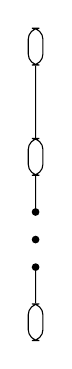
\begin{tikzpicture}[>=latex,scale=0.7]
\scriptsize
\draw (5,4) node[draw,rounded corners,align=left] (a) {\\};
\draw (5,2) node[draw,rounded corners,align=left] (b) {\\};
\draw (5,-1) node[draw,rounded corners,align=left] (c) {\\};
\draw [-] (a) --(b);
\draw [-] (b)  -- (5,1);
\draw [-] (c) -- (5,0);
\fill (5,1) circle (0.07cm);
\fill (5,0.5) circle (0.07cm);
\fill (5,0) circle (0.07cm);
\end{tikzpicture}
}
  \caption{Tree decomposition of the layered graph with  layers of
    width  each}
  \label{fig:layertree}
\end{figure}
Observe that in the  run of the loop written in lines
-- Algorithm~\ref{algo:layer} computes the cost of embedding
all the edges and nodes present in the vertex  of the tree
decomposition for all possible mappings of nodes in  In lines
-- the algorithm finds the optimal embedding cost of all the
nodes and edges till  conditioned on the mapping of vertices in
 Lines -- compute the cost till the last
layer and then the algorithm traces back from  to  to
get the final optimal cost and the corresponding embedding (lines
-). Note that the time required to compute the cost till
vertex  depends on the size of this vertex (lines  define
that value). And the total time to complete the process can be written
as  where  is the size of largest  in a tree
decomposition.

Therefore if we can find the tree decomposition of any computation
graph  of  vertices with size of largest vertex to be
 then an algorithm similar to Algorithm~\ref{algo:layer} can be
used to compute the minimum cost embedding in time 

\begin{figure}[tbp]
\centering
\subfloat[]{
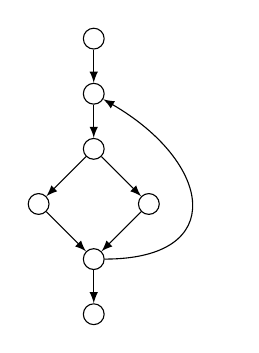
\begin{tikzpicture}[>=latex,scale=0.7]
 \scriptsize
 \tikzstyle{every node} = [circle,draw=black]
\node (s) at (0,3) {};
 \node (a) at (0,2) {};
 \node (b) at (0,1) {};
 \node (c) at (-1,0) {};
 \node (d) at (1,0) {};
 \node (e) at (0,-1) {};
 \node (t) at (0,-2) {};
\draw [->] (s) -- (a);
 \draw [->] (a) --(b);
 \draw [->] (b) --(c);
 \draw [->] (b) --(d);
 \draw [->] (c) --(e);
 \draw [->] (d) --(e);
 \draw [->] (e) --(t);   
 \draw [->] (e) to[out=0,in=-30,looseness=2] (a);
\end{tikzpicture}
}
\hspace*{10pt}
\subfloat[]{
\begin{tikzpicture}[>=latex,scale=0.7]
  \scriptsize
  \tikzstyle{every node} = [circle,draw=black]
  \node (a) at (0,3) {};
  \node (b) at (0,1) {};
  \node (c) at (2,-1) {};
  \node (d) at (1,-3) {};
  \node (e) at (-2,-1) {};
\draw [-] (a) -- (b) -- (c) -- (d);
  \draw [-] (b) -- (e);
\end{tikzpicture}
} 
 \caption{(a). A simple computation graph with directed
    cycle. (b). Tree decomposition of the graph}
  \label{fig:series}
\end{figure}

An example of a non DAG graph for the technique discussed above is
shown in Fig.~\ref{fig:series}a. It is a computation
schema that has a conditional jump, represented by the link between
vertexes  and . This is an example of a series-parallel graph
\cite{Diestel00} and such graphs are amenable to a tree decomposition
like in Fig.~\ref{fig:series}b.  In the preceding we have shown that
the technique used in Algorithm~\ref{algo:layer} can also be used to
find the minimum cost embedding of a series-parallel computation
graph, among others, that can have a bounded tree decomposition.

\section{Updating Solution to \mincost\ for Perturbations of }
\label{sec:change_computation}

Let us consider a situation where the minimum cost embedding for a
layered graph  is given and one needs to find the
embedding for a new graph  which is generated by
adding vertices and/or edges in  We assume that
 is still a layered graph with  layers and
maximum width  Assume that we are given a set of  tuples
 where edge  is added at layer  Note that edge
 should have at least one end point at the existing vertex in
graph  To find the new embedding we first sort the 
tuples in  such that  Now we start adding the edges layer wise from 
to  At any layer  the following three types of additions are
possible.

\begin{enumerate}
\item \textbf{Addition of a vertex with only one edge.} When a vertex,
  say  is added with an edge  to an existing vertex  at
  layer  then  can be seen as a sink to an intermediate
  function value available at  Let us assume that the vertex 
  is mapped to vertex  under the original
  embedding. If the mapping  of  is predefined
  (which is generally the case for all the sources and sinks in the
  network) then we just have to find the minimum cost path between
   and  and add it to the existing embedding to find the new
  embedding. If the mapping of  is not predefined then mapping it
  to  will give the minimum cost embedding. This can be done in
   time.

\item \textbf{Addition of an edge between two existing vertices.} Let
  us consider a situation when an edge  is added such that  is
  at layer  and  is at layer  with weight 
  The data structure already available for each layer  after
  running Algorithm~\ref{algo:layer} is shown in
  Fig.~\ref{fig:algo}. Recall that  is the cost of
  embedding till layer  (including the edges between layer  and
  ) when vertices of layer  are at  and that of 
  are at  And  is the optimal cost till layer  when
  vertices at layer  are at  If the vertex  is placed
  at  and  is placed at  then the new
  cost of embedding is  (line number  of
  Algorithm~\ref{algo:layer}). One needs to modify the whole 
  matrix at layer  by adding a value and correspondingly the
  minimum cost  will also change (line number ). As
  the value of  changes the pointers to compute  the
  values for all the subsequent layers will also change. Hence at each
  layer  we will modify the whole data structure just by adding new
  values of  and subtracting the old values of 
  Once all the data structures are changed the algorithm needs to run
  the same back tracking procedure (lines -- to get the new
  embedding. Assuming that the modification in the data structure at
  each layer can be done in  time then the new embedding can be
  found in  time.

\item \textbf{Addition of a vertex with more than one edge.} Let a
  vertex  is added to layer  with more than one edges to
  existing vertices at layer  and/or  The width of the
  layer  is still upper bounded by  By following the same logic
  presented above it is easy to observe that now the data structures
  from layer  onward will change, i.e.,  and
   will also change. And the new embedding can again be
  found in  time.
\end{enumerate}

Note that at a layer  the data structure changes due to edges added
to layers  (which takes  time) and the edge
added at layer  (which takes only  time as described
earlier). Hence the total time to change all the data structures in
this process will be just  where  is the total number of
layers, as opposed to  if we add each edge separately.
\begin{figure}[tbp]
  \centering
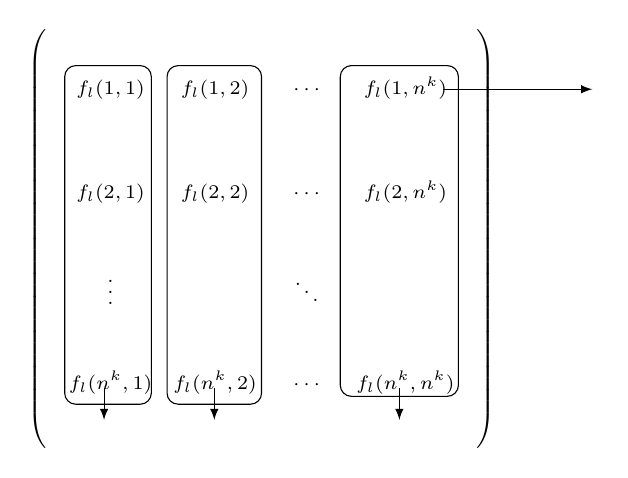
\begin{tikzpicture}[>=latex]
\scriptsize
 \matrix (A) [matrix of math nodes,nodes = {node style ge},left delimiter  = (,right delimiter = )] at (0,0)
             {
 f_l(1,1) & f_l(1,2) & \cdots & f_l(1,n^k) \\
 f_l(2,1) & f_l(2,2) & \cdots & f_l(2,n^k) \\
 \vdots & & \ddots \\
 f_l(n^k,1) & f_l(n^k,2) & \cdots & f_l(n^k,n^k) \\
};
 \draw [->] (2.3,1.9) -- (4.2,1.9);
 \node at (4.2,1.9) [draw=none,above] {};

 \draw [rounded corners] (1,-2) rectangle (2.5,2.2);
 \draw [->] (1.75,-1.9) -- (1.75,-2.3);
 \node at (1.75,-2.3) [draw=none,below] {};
 
 \draw [rounded corners] (-2.5,-2.1) rectangle (-1.4,2.2);
 \draw [->] (-2,-1.9) -- (-2,-2.3);
 \node at (-2,-2.3) [draw=none,below] {};  
 
  \draw [rounded corners] (-1.2,-2.1) rectangle (0,2.2);
  \draw [->] (-0.6,-1.9) -- (-0.6,-2.3);
 \node at (-0.6,-2.3) [draw=none,below] {};
\end{tikzpicture}
 \caption{Data structure in Algorithm~\ref{algo:layer} at layer }
  \label{fig:algo}
\end{figure}



\section{Discussion}
\label{sec:discuss}

\subsection{Distributed versions of the algorithms.}  

Note that Algorithms~\ref{algo:tree} and \ref{algo:layer} are both
centralized algorithms. In other words they both need knowledge of
 The algorithms have two stages with the all-pair distance
matrix  of  computed in the first stage and the
optimal value of  and  using  computed in the
second stage; see lines  and  of algorithm~\ref{algo:tree} and
lines  and  of Algorithm~\ref{algo:layer}.  Observe that once
 is known, the outputs of our algorithms are independent
of the vertex of the communication network which runs the
algorithm. Hence all vertices in  can run the algorithms to
obtain the optimal embedding without interacting with the other
vertices in the network. Hence if one can compute the distance matrix
in a distributed way in the network, then the optimal embedding can
also be found in a distributed manner. Several distributed algorithms
to find  are available, e.g., \cite{Kanchi04}.

\subsection{Delay in the network with bounded capacity.}

In Section~\ref{sec:prelims} we discussed \mindelay\ which finds the
minimum delay embedding of  on  The delay
calculation in \eqref{eq:nodedelay} (Section~\ref{sec:prelims}, Page
 assumes that each edge  has infinite
capacity and can transmit as much data as needed in time  where
 is the delay of an edge  In general the edges in the
network have finite capacity and can transmit only one type of data in
time  Here we describe the delay in the network in the general
setting. Recall that an edge  is mapped to a
path in  in embedding  (defined in
Definition~\ref{def:embedding}). Delay of a network edge  is the
time required for data to go from  to  We say that an edge
 has arrived at link  when the data
corresponding to  is ready for transmission on  at vertex
 Similarly, we say that the edge  has departed from link
 when the data reaches  via link  Let there be  edges
 of  mapped to an edge  under embedding  Let the arrival time of these
edges at the link  be  We assume that the capacity of each link is such
that at a given time only one kind of data can be transmitted over it
in the network. Then the departure time of these edges from the link
will be  The
departure from the link  can be calculated recursively as follows:

Let an edge  be mapped to
a path  in  under embedding 
such that  and  Then the delay of  in the embedding is the sum of the
delay incurred at each link  which
can be written as:
 
Now the delay of a vertex  in the embedding  can
be defined as \eqref{eq:nodedelay} where
 in computed as the
above equation. We explain our point by an example.
\begin{example}
  \label{ex:delay}
  Consider a computation graph and a communication graph shown in
  Fig.~\ref{fig:delay}. We consider that there are processing delays
  and delay associated with each edge of the communication graph is
   Consider an embedding  such that  Similarly,  It is easy to observe
  that using the delay model described in the
  Section~\ref{sec:prelims} the delay of the embedding is  While
  in the model described above as the embedding of edges  and
   have a common edge  in them the delay of the embedding
  increases to 
\begin{figure}[tbp]
    \centering
\subfloat[]{
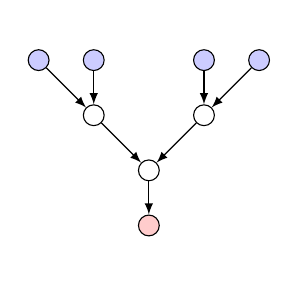
\begin{tikzpicture}[>=latex,scale=0.7]
 \scriptsize
 \tikzstyle{every node} = [circle,draw=black]
 \node (a) at (-2,0) [fill=blue!20] {};
 \node (b) at (-1,0) [fill=blue!20] {};
 \node (h) at (1,0) [fill=blue!20] {};
 \node (c) at (2,0) [fill=blue!20] {};
 \node (d) at (-1,-1)[font=\tiny]  {};
 \node (e) at (1,-1) [font=\tiny]{};
 \node (f) at (0,-2)[font=\tiny] {};
 \node (g) at (0,-3) [fill=red!20]{};
 \node at (-2,0.4) [draw=none]{};
 \node at (-1,0.4) [draw=none]{};
 \node at (1,0.4) [draw=none]{};
 \node at (2,0.4) [draw=none]{};
 \node at (0,-3.4) [draw=none]{};
 \node at (d) [draw=none,right=4pt] {};
 \node at (e) [draw=none,right=4pt] {};
 \node at (f) [draw=none,right=4pt] {};
\draw [->] (a) -- (d) ;
 \draw [->] (b) -- (d) ;
 \draw [->] (h) -- (e) ;
 \draw [->] (c) -- (e) ;
 \draw [->] (d) -- (f) ;
 \draw [->] (e) -- (f) ;
 \draw [->] (f) -- (g) ;
\end{tikzpicture}
}
\hspace*{10pt}
\subfloat[]{
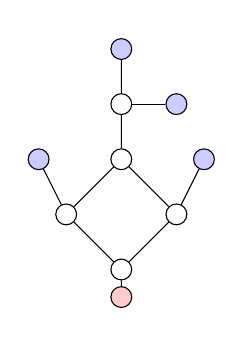
\begin{tikzpicture}[>=latex,scale=0.7]
  \scriptsize
  \tikzstyle{every node} = [circle,draw=black]
  \node (a) at (0,2) [fill=blue!20] {};
  \node (b) at (0,1) {};
  \node (c) at (1,1) [fill=blue!20] {};
  \node (d) at (0,0) {};
  \node (e) at (-1,-1) {};
  \node (f) at (1,-1) {};
  \node (g) at (-1.5,0) [fill=blue!20] {};
  \node (h) at (1.5,0) [fill=blue!20] {};
  \node (i) at (0,-2) {};
  \node (j) at (0,-2.5) [fill=red!20] {};  
\draw [-] (a) -- (b) -- (d) -- (e) -- (i) -- (j);
 \draw [-] (c) -- (b);
 \draw [-] (g) -- (e);
 \draw [-] (d) -- (f) -- (i);
 \draw [-] (h) -- (f); 
\node at (a) [draw=none,above] {};
  \node at (c) [draw=none,above] {};
  \node at (g) [draw=none,above] {};
  \node at (h) [draw=none,above] {};
  \node at (j) [draw=none,below] {};
  \node at (b) [draw=none,left] {};
  \node at (d) [draw=none,left] {};
  \node at (e) [draw=none,left] {};
  \node at (f) [draw=none,left] {};
  \node at (i) [draw=none,left] {};
\end{tikzpicture}
} 
  \caption{(a) Computation graph for function .  (b) Communication Network where every
      edge has delay }
    \label{fig:delay}
  \end{figure}
\end{example}

As mentioned in Example~\ref{ex:delay} the actual delay is more than
the delay defined by \eqref{eq:nodedelay} when multiple edges of
 are mapped to one edge of  in an embedding. We
study the impact of our assumption via simulations.

We studied the behavior of minimum delay embedding and find the
statistics on maximum number of times an edge of  is used in the
minimum delay embedding of a typical  In our study the
computation graph was taken to be a binary tree of  vertices and
its minimum delay embedding on a random graph of  vertices was
calculated using Algorithm~\ref{algo:tree}. The probability of an edge
being present in the random graph ( was varied from  to
 Note than as  increases the number of edges in the network
increases. The communication and transmission costs were assumed to be
one and the processing cost was chosen uniformly from integers
 For each value of   instances of network were
generated and for each instance Algorithm~\ref{algo:tree} was run for
 random initial placements of sources and sink. The mean and the
median of the maximum number of times an edge in the network graph is
used in the embedding for each  is shown in
Fig.~\ref{fig:meantree}. Observe that as the number of edges are
increased in the network maximum number of times an edge is used
converges to one. Hence we can say that for the networks with large
number of edges compared to that of the computation graph our
assumption of delay calculated by \eqref{eq:nodedelay} will be same as
that of delay computed by \eqref{eq:actualdelay}.

\begin{figure}[tbp]
  \centering
  \includegraphics[width=\linewidth]{tree_stat.pdf}
  \caption{Statistics for maximum number of times a link is used in
    minimum delay embedding}
  \label{fig:meantree}
\end{figure}

\bibliographystyle{IEEE}
\bibliography{function-computation}


\appendices

\section{Hardness PCS-FM}
\label{sec:PCS-FM}

Here we prove that PCS-FM problem is NP-complete by reducing it to
another NP-complete problem \textit{Precedence Constraint Scheduling
  (PCS)} \cite{Garey79}.

PCS problem is defined as follows. Given a set  of tasks
with a  partial order on it each having length
 and 
processors then find a schedule  of tasks on processors which
meets an overall deadline  and obeys the precedence
constraints, i.e., if for some   then 

First we define an instance of PCS-FM problem  from an instance of PCS problem  We
create partial order graph  from  as
shown in Fig.~\ref{fig:scheduling}. The graph  has two
parts: One part is the same as  and the other part
has  new vertices  giving  The vertices  are connected
to  by a directed edge and  is connected to all the vertices
of  Note that as all the edges are going away from 
the new graph is still a DAG. Let  and  Define  and
 for all  Let us number the
processors from  to  as  Let us define  and the deadline for  is 

To prove our claim we have to show that there exists a schedule
 for  which meets the deadline  if
and only if there exists a schedule  for  which meets
the deadline  Now observe that in any schedule  for 
any task in  cannot start unless task  is finished
which in turn cannot start unless all the tasks 
are finished. As it is given that the tasks  go to
separate processors (due to  they all can be finished in 
time step giving  Similarly
 for all  Hence
if there is a schedule  for  which starts at
 and finishes before  then a schedule  for  can be
defined as  for all 
 for all  and  It is
easy to observe that this is a valid possible schedule and finishes
before 

\begin{figure}[tbp]
  \centering
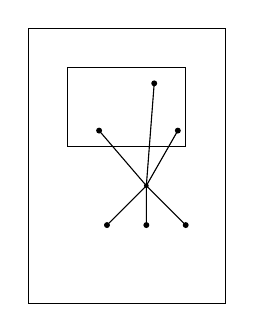
\begin{tikzpicture}[>=latex]
\draw (0.5,1) rectangle (2,2);
\footnotesize;
\node at (1.2,1.7) {};
\fill (1.5,0.5) circle (0.03cm);
\node at (1.9,0.5) {};
\draw [->] (1.5,0.5) -- (0.9,1.2) [fill] circle (0.03cm);
\draw [->] (1.5,0.5) -- (1.6,1.8) [fill] circle (0.03cm);
\draw [->] (1.5,0.5) -- (1.9,1.2) [fill] circle (0.03cm);
\draw [->] (1.5,0.5) -- (1,0) [fill] circle (0.03cm);
\draw [->]  (1.5,0.5) -- (1.5,0) [fill] circle (0.03cm);
\draw [->] (1.5,0.5) -- (2,0) [fill] circle (0.03cm);
\node at (1,-0.3) {};
\node at (1.5,-0.3) {};
\node at (2,-0.3) {};
\draw (0,-1) rectangle (2.5,2.5);
\node at (2.7,2.4) {};
\end{tikzpicture}
 \caption{Transformation of PCS into PCS-FM problem}
  \label{fig:scheduling}
\end{figure}


To complete the proof we have to prove that if there is no schedule
for  which finishes before  then there is no
schedule for  which finishes before  We prove
this by contradiction. Let us assume that there is a schedule 
for  which finishes before  but there is no schedule for
 which finishes before  As noted earlier in any
schedule for  first two time slots are required to finish tasks
 and then only any other task can start. So in the
schedule  for all  Total
time taken to finish the tasks of  is  It means that there is a mapping of
tasks of  on  processors such that the total time to
finish is less than  which implies that there is a
schedule for  which finishes before the deadline 
This is a contradiction to our assumption. Hence it is proved that the
problem PCS-FM is as hard as PCS.


\end{document}